\section{Offline Rule Generator}
\label{sec:rule_generator}
The Rule Generator turns LLM rewrites into verified rules using Algorithm~\ref{alg:pipeline}.
We sample workload queries and rewrite them with an LLM rewriter (Section~\ref{sec:offline:sample}).
Furthermore, we distill each rewrite into candidate rules (Section~\ref{sec:offline:distill}), generate C++ for each rule (Section~\ref{sec:offline:implement}), as well as verify and integrate each rule (Section~\ref{sec:offline:verify}).


\begin{algorithm}[b]\fontsize{7.9}{0}
\caption{Rule Generation Pipeline}
\label{alg:pipeline}
\begin{algorithmic}[1]
\REQUIRE workload $\mathcal{W}$, LLM $\mathcal{M}$, database $\mathcal{D}$, SMT budget $B_{\mathit{smt}}$
\ENSURE rule set $\mathcal{R}$, Fragment Index $\mathit{FI}$, rule ordering $\omega$
\STATE \label{pipeline:sample} $\mathcal{Q}_s \leftarrow \textsf{Sample}(\mathcal{W})$;\quad $\mathcal{D}_s \leftarrow \textsf{Downsample}(\mathcal{D})$
\FOR{$Q \in \mathcal{Q}_s$}
  \STATE \label{pipeline:rewrite} \blue{$Q'' \leftarrow \textsc{Rewriter}(Q)$} \algorithmiccomment{\blue{rewritten SQL}}
  \IF{$Q'' = Q$}
    \STATE \label{pipeline:skip} \textbf{continue} \algorithmiccomment{no transformation found}
  \ENDIF
  \FOR{\label{pipeline:distill} \blue{$r^* \in \textsf{Distill}(Q,\, Q'')$} \textbf{not in} $\mathcal{R}$}
    \STATE \label{pipeline:implement} $r_{\mathit{impl}} \leftarrow \textsf{Implement}(r^*,\, \mathcal{M})$ \algorithmiccomment{LLM writes C++ rule}
    \STATE \label{pipeline:verify} $(\mathit{ok},\, \mathit{fb}) \leftarrow \textsf{Verify}(r_{\mathit{impl}},\, \mathcal{R},\, \mathcal{Q}_s,\, \mathcal{D}_s)$; $\mathit{k} \leftarrow 0$
    \WHILE{$\lnot\,\mathit{ok}$ \AND $\mathit{k} < \textsc{MaxRetries}$}
      \STATE $r_{\mathit{impl}} \leftarrow \textsf{Implement}(\textsf{FixPrompt}(r^*,\, \mathit{fb}),\, \mathcal{M})$; $\mathit{k} \leftarrow \mathit{k}+1$
      \STATE \label{pipeline:retry} $(\mathit{ok},\, \mathit{fb}) \leftarrow \textsf{Verify}(r_{\mathit{impl}},\, \mathcal{R},\, \mathcal{Q}_s,\, \mathcal{D}_s)$
    \ENDWHILE
    \IF{$\mathit{ok}$}
      \STATE \label{pipeline:integrate} $\mathcal{R} \leftarrow \mathcal{R} \cup \{r_{\mathit{impl}}\}$; register $\mathcal{K}_{r_{\mathit{impl}}}$ in $\mathit{FI}$ \algorithmiccomment{hot-reload}
    \ENDIF
  \ENDFOR
\ENDFOR
\STATE \label{pipeline:order} \blue{$\omega \leftarrow \textsf{SortByPriority}(\mathcal{R})$} \algorithmiccomment{\blue{default order,} Section~\ref{sec:online:apply}}
\RETURN $\mathcal{R},\, \mathit{FI},\, \omega$
\end{algorithmic}
\end{algorithm}

\vspace{-0.1cm}
\subsection{Sampling and Rewriting}
\label{sec:offline:sample}
The pipeline starts from a sample $\mathcal{Q}_s \subseteq \mathcal{W}$ of $n$ queries and a downsampled database $\mathcal{D}_s$ for testing (Line~\ref{pipeline:sample}).
Two channels feed the query sample.
The \emph{performance-driven} channel monitors execution time, cardinality estimates, and plan shape, and flags queries that a rewrite could speed up. Additionally, administrators may flag queries that are business-critical.
\blue{In our experiments, $\mathcal{Q}_s$ holds 5 queries each for Stats-CEB, JOB-Complex, TPC-H, and IMDB Full, 6 for JOB, 11 for DSB, and 8 of the 1,190 StackOverflow queries.}
% TODO(Saeed, Q4): if the five selected queries per workload match the five slowest on the host, add:
% "The performance-driven channel selects the five slowest queries on the host."
% Otherwise, state the actual criterion openly and list rerunning with host-latency selection as a limitation.
For each sampled query $Q$, an LLM rewriter\footnote{The LLM rewriter is pluggable; any whole-query rewriters \cite{GenRewrite,resequel} are applicable.} returns its best rewrite $Q''$ as SQL only (Line~\ref{pipeline:rewrite}); the transformations are distilled from the query pair.
If $Q'' = Q$, the rewriter found no transformation, and the pipeline moves to the next query (Line~\ref{pipeline:skip}).


\subsection{Rule Distillation}
\label{sec:offline:distill}
Distillation extracts from a query pair $(Q, Q'')$ rules that transfer to other queries.
It works on logical plans, not on SQL text, which enables two kinds of generalization.
\emph{Value independence} removes predicate constants, column and table names, and keeps operator types and tree shape.
\emph{Arity independence} parameterizes the pattern over the number of joined tables $N$, so a rules distilled from three-table joins also fire on four-table joins with the same shape.

\textbf{Algorithm Details:} Algorithm~\ref{alg:distill} shows the procedure.
Lines~\ref{distill:parseQ}--\ref{distill:parseQr} parse $Q$ and $Q''$ into logical plans $P$ and $P''$.
If the plans are identical, the rewrite changed only the SQL text, and the pair yields no rule (Line~\ref{distill:identical}).
Line~\ref{distill:diff} computes $\Delta$, the operator-level difference between $P$ and $P''$ in terms of added, removed, and reordered/restructured operators and predicates.
Since rewrites often combine several changes---such as a new aggregate and a new join order---Line~\ref{distill:split} splits $\Delta$ into these changes. Lines~\ref{distill:diff}--\ref{distill:split} are a single LLM call that compares $P$ and $P''$ and returns one entry per change, each labeled with the most specific Apache Calcite rule; or if none matches, a custom identifier (e.g., \texttt{PREDICATE\_\allowbreak RANGE\_\allowbreak TO\_\allowbreak BETWEEN}). The same call discards changes that are not semantics-preserving or purely syntactic (e.g., on Stats-CEB, it discards 25 and 21 of the 146 pairs and splits the rest into 415 changes with 30 labels). The algorithm distills one rule per change $\delta$, and equivalent changes across queries yield the same rule.
% TODO(Saeed, Q2): does SplitChanges follow the transformations named in E? Which of the steps below are LLM calls?
For each $\delta$, an LLM derives the applicability condition $\phi$ and the transformation $\tau$ (Lines~\ref{distill:pattern}--\ref{distill:transform}).
Both refer to operator roles, such as the anchor table and its branches, not to concrete tables or constants.
If $\phi$ or $\tau$ is empty or cannot be expressed in the rule language, $\delta$ yields no rule (Line~\ref{distill:degenerate}).
Otherwise, Line~\ref{distill:keys} extracts the fragment keys $\mathcal{K}$ from $\phi$ and adds the candidate rule $(\phi, \tau, \mathcal{K})$.
Each candidate takes the priority that the LLM assigns when it derives the rule, which sets the default rule order (Section~\ref{sec:online:apply}).
We keep only new candidates (Line 6 of Algorithm~\ref{alg:pipeline}), and discard equivalent ones, also across workloads.
Overlapping rules (that make the same change but in a different way) may still remain though.
Overlapping rules (that make the same change but in a different way) may still remain though.
Overlapping rules (that make the same change but in a different way) may still remain though.\shorten

\begin{algorithm}[t]\fontsize{7.9}{9.5}\selectfont
\caption{\textsf{Distill}$(Q, Q'')$: Candidate Rule Extraction}
\label{alg:distill}
\begin{algorithmic}[1]
\REQUIRE original query $Q$, rewritten query $Q''$
\ENSURE set of candidate rules $\mathcal{R}^*$, each $r^* = (\phi,\, \tau,\, \mathcal{K})$
\STATE \label{distill:parseQ} $P \leftarrow \textsf{ParseToPlan}(Q)$
\STATE \label{distill:parseQr} $P'' \leftarrow \textsf{ParseToPlan}(Q'')$
\IF{\label{distill:identical} $P = P''$}
  \RETURN $\varnothing$ \algorithmiccomment{identical plans}
\ENDIF
\STATE \label{distill:diff} \blue{$\Delta \leftarrow \textsf{StructuralDiff}(P,\, P'')$} \algorithmiccomment{\blue{plan difference (LLM)}}
\STATE $\mathcal{R}^* \leftarrow \varnothing$
\FOR[\blue{labeled independent changes}]{\label{distill:split} $\delta \in \textsf{SplitChanges}(\Delta)$}
  \STATE \label{distill:pattern} $\phi \leftarrow \textsf{GeneralizePattern}(\delta)$ \algorithmiccomment{applicability condition}
  \STATE \label{distill:transform} $\tau \leftarrow \textsf{GeneralizeTransform}(\delta)$ \algorithmiccomment{transformation}
  \IF{\label{distill:degenerate} $\phi \neq \varnothing$ \AND $\tau \neq \varnothing$}
    \STATE \label{distill:keys} $\mathcal{K} \leftarrow \textsf{ExtractFragmentKeys}(\phi)$
    \STATE $\mathcal{R}^* \leftarrow \mathcal{R}^* \cup \{(\phi,\, \tau,\, \mathcal{K})\}$
  \ENDIF
\ENDFOR
\RETURN \label{distill:return} $\mathcal{R}^*$
\end{algorithmic}
\end{algorithm}

\begin{figure*}[t]
\vspace{-0.25cm}
    \centering
    \resizebox{.99\textwidth}{!}{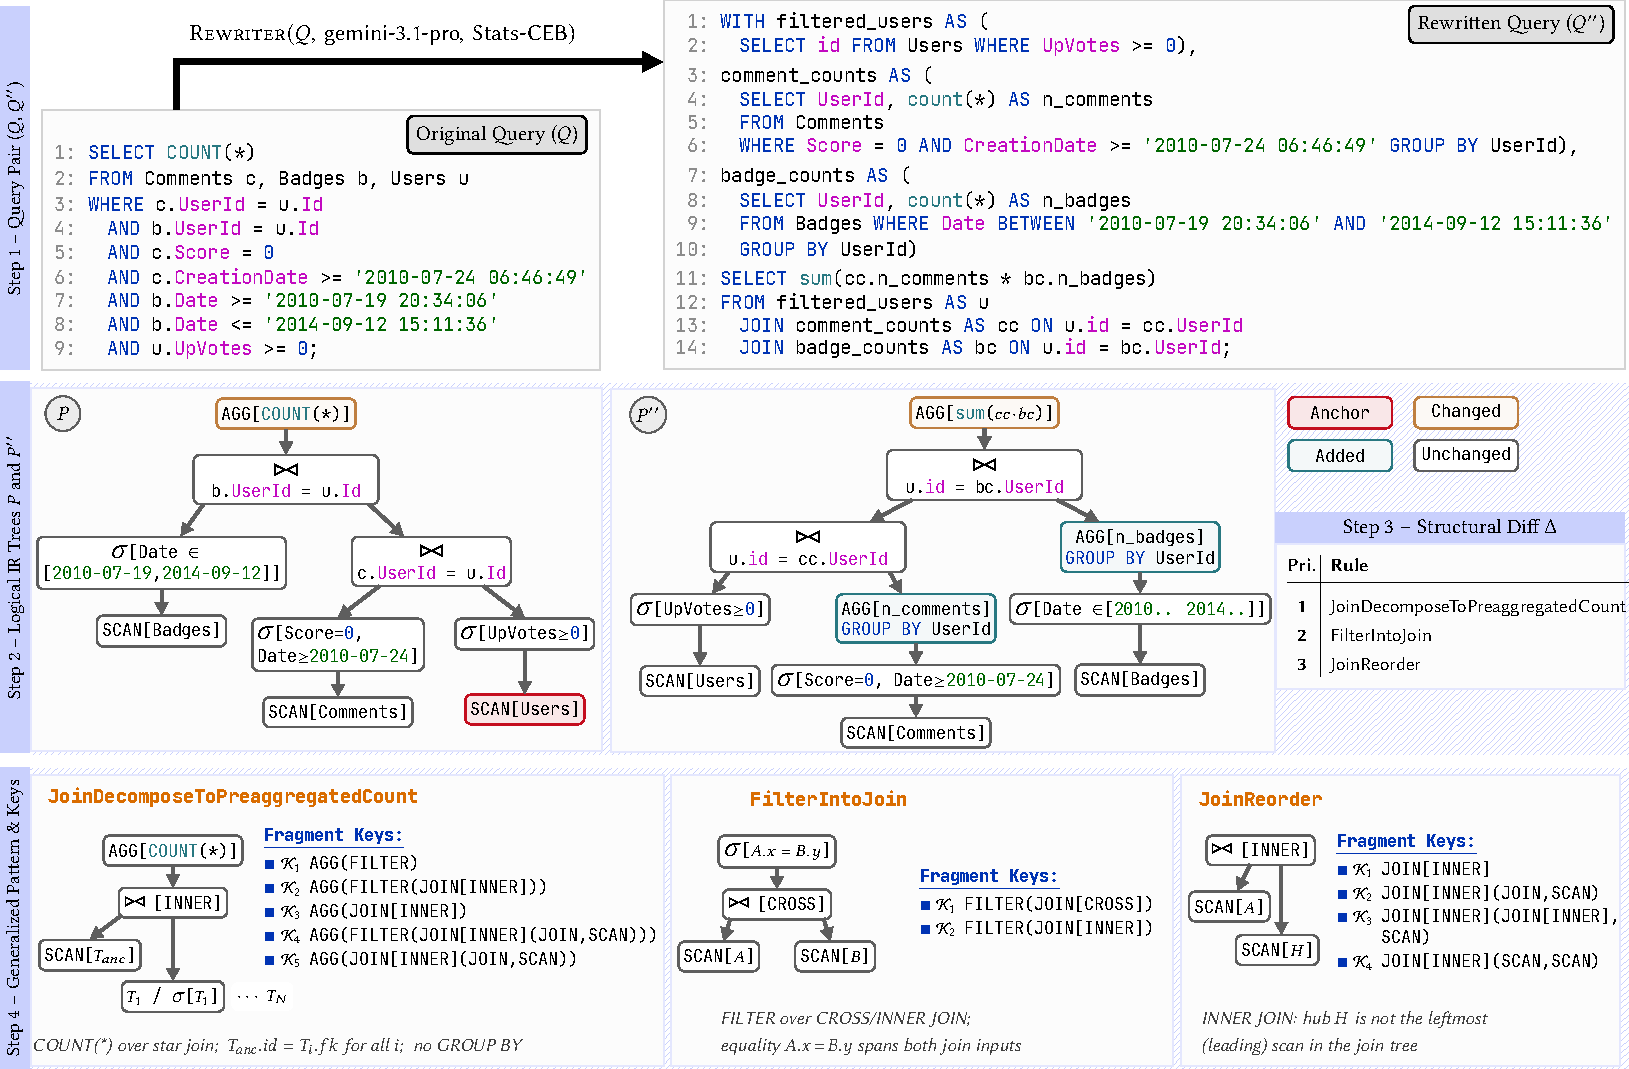
\includegraphics[scale=1]{figures/img/fig_StatsQ88}}
    \vspace{-0.35cm}
    \caption{Distilling rules from Stats-CEB query~88: (1) query pair $(Q, Q'')$ from the LLM rewriter, (2) logical plans with anchor, added, and changed operators, (3) three candidate rules ranked by priority, (4) generalized patterns and fragment keys.}
    \label{fig:distill:example}
    \vspace{-0.4cm}
\end{figure*}


\begin{example}[Rule Distillation]\label{ex:1}
\emergencystretch=3em
Figure~\ref{fig:distill:example} traces Algorithm~\ref{alg:distill} on Stats-CEB query~88.
\emph{Step~1, query pair:}
Query~88 counts the rows of joining \texttt{Comments}, \texttt{Badges}, and \texttt{Users}, all on \texttt{UserId}.
The rewriter decomposes this join into three CTEs.
\texttt{filtered\_users} applies the filter on \texttt{Users}.
\texttt{comment\_counts} and \texttt{badge\_counts} count the matching rows per user in each branch.
The root computes \texttt{SUM(n\_comments} $\times$ \texttt{n\_badges)}.
\emph{Step~2, logical plans (Lines~\ref{distill:parseQ}--\ref{distill:parseQr}):}
In both plans, \texttt{Users} is the anchor table.
$P''$ adds one pre-aggregation \texttt{AGG[COUNT(*) GROUP BY UserId]} per branch and turns the root \texttt{COUNT} into a \texttt{SUM}.
\emph{Step~3, difference (Lines~\ref{distill:diff}--\ref{distill:split}):}
The LLM splits $\Delta$ into seven changes, and three candidate rules, in priority order.
\texttt{JoinDecomposeTo\allowbreak Preaggregated\allowbreak Count} captures the new pre-aggregation and root aggregate.
\texttt{FilterIntoJoin} captures the moved join predicates \texttt{c.UserId = u.Id} and \texttt{b.UserId = u.Id} from the \texttt{WHERE} to the \texttt{ON} clauses (\texttt{FILTER\_\allowbreak INTO\_\allowbreak JOIN}).
\texttt{JoinReorder} captures the new join order, which starts from the anchor scan (\texttt{JOIN\_REORDER}).
The remaining changes prune unused columns, materialize the filter on \texttt{Users}, and rewrite a range predicate as \texttt{BETWEEN}; they yield smaller rules omitted here.
\emph{Step~4, generalization (Lines~\ref{distill:pattern}--\ref{distill:keys}):}
Each rule refers to operator roles (an anchor and $N$ branches, a hub $H$, or two join inputs $A$ and $B$), not concrete tables.
Its fragment keys, such as \texttt{AGG(JOIN[INNER])}, let the Fragment Index retrieve the rule for any query with this fragment, and $\phi$ then checks the full shape.\shorten
\end{example}


\begin{algorithm}[t]\fontsize{7.9}{0}
\caption{\textsf{Verify}$(r_{\mathit{impl}}, \mathcal{R}, \mathcal{Q}_s, \mathcal{D}_s)$}
\label{alg:verify}
\begin{algorithmic}[1]
\REQUIRE rule $r_{\mathit{impl}}$, rule set $\mathcal{R}$, sample $\mathcal{Q}_s$, downsampled database $\mathcal{D}_s$, SMT budget $B_{\mathit{smt}}$
\ENSURE $\mathsf{valid}$ or $(\mathsf{invalid},\, \mathit{feedback})$
\COMMENTLINE{Stage 1: smoke test}
\IF{\label{verify:compile} $\lnot\,\textsf{Compile}(r_{\mathit{impl}})$}
  \RETURN $(\mathsf{invalid},\;\textsf{CompileError}(r_{\mathit{impl}}))$
\ENDIF
\IF{\label{verify:smoke} $\lnot\,\textsf{SmokeCheck}(r_{\mathit{impl}})$}
  \RETURN $(\mathsf{invalid},\;\textsf{PatternMismatch}(r_{\mathit{impl}}))$
\ENDIF
\COMMENTLINE{Stage 2: formal check under budget $B_{\mathit{smt}}$}
\STATE \label{verify:smt} $\mathit{res} \leftarrow \textsf{SMT.Check}(Q,\, r_{\mathit{impl}}(Q),\, B_{\mathit{smt}})$ \algorithmiccomment{\blue{$Q$: source query of $r_{\mathit{impl}}$}}
\IF{\label{verify:eq} $\mathit{res} = \mathsf{EQ}$}
  \RETURN $\mathsf{valid}$ \algorithmiccomment{proven equivalent}
\ELSIF{\label{verify:neq} $\mathit{res} = \mathsf{NEQ}$}
  \RETURN $(\mathsf{invalid},\;\textsf{Counterexample}(\mathit{res}))$
\ENDIF
\COMMENTLINE{Stage 3: result-equivalence test ($\mathit{res} = \mathsf{UNKNOWN}$ or $\mathsf{ERROR}$)}
\STATE $\mathcal{R}' \leftarrow \mathcal{R} \cup \{r_{\mathit{impl}}\}$;\quad$\Sigma \leftarrow \emptyset$;\quad$\mathcal{Q}_{\mathit{sel}} \leftarrow \emptyset$
\FOR{\label{verify:dedup} $Q \in \mathcal{Q}_s$}
  \STATE $s \leftarrow \textsf{FiringSequence}(\mathcal{R}', Q)$
  \IF{$s \notin \Sigma$}
    \STATE $\Sigma \leftarrow \Sigma \cup \{s\}$;\quad$\mathcal{Q}_{\mathit{sel}} \leftarrow \mathcal{Q}_{\mathit{sel}} \cup \{Q\}$ \algorithmiccomment{one query per sequence}
  \ENDIF
\ENDFOR
\IF{\label{verify:nofire} no $Q \in \mathcal{Q}_{\mathit{sel}}$ fires $r_{\mathit{impl}}$}
  \RETURN $(\mathsf{invalid},\;\textsf{NotExercised}(r_{\mathit{impl}}))$
\ENDIF
\FOR{\label{verify:exec} $Q \in \mathcal{Q}_{\mathit{sel}}$}
  \STATE $Q_{\mathit{rw}} \leftarrow \textsf{Rewrite}(Q,\, \mathcal{R}')$ \algorithmiccomment{priority order}
  \IF{$\textsf{Exec}(\mathcal{D}_s, Q) \neq \textsf{Exec}(\mathcal{D}_s, Q_{\mathit{rw}})$}
    \RETURN $(\mathsf{invalid},\;Q,\;\textsf{FiringSequence}(\mathcal{R}', Q))$
  \ENDIF
\ENDFOR
\RETURN $\mathsf{valid}$
\end{algorithmic}
\end{algorithm}


\begin{table*}[t]
\centering
\caption{Ten of the 16 verified rules that {\sys} generates for Stats-CEB, sorted by descending priority (Pri.). The Calcite column marks whether Apache Calcite has an equivalent rule: \cmark~exact, $\sim$~partial, \xmark~none. Seven of the ten rules have none.}
\vspace{-.35cm}
\label{tab:rules:statsceb}
\small
\begin{tabular}{rlrp{0.52\textwidth}c}
\toprule
\textbf{\#} & \textbf{Rule} & \textbf{Pri.} & \textbf{Transformation} & \textbf{Calcite} \\
\midrule
1  & \texttt{AggregateDecomposeCrossJoin}       & 80 & \texttt{COUNT(*)} over an $N$-way implicit cross join $\to$ partial-count CTEs & \xmark \\
2  & \texttt{AggregateDecomposeMultiHub}        & 79 & \texttt{COUNT(*)} over a two-level star join $\to$ per-branch CTEs & \xmark \\
3  & \texttt{JoinDecomposeToPreaggregatedCount} & 70 & \texttt{COUNT(*)} over a multi-branch join $\to$ pre-aggregated CTEs per branch & \xmark \\
4  & \texttt{JoinEliminateViaFK}                & 60 & Remove a bridge table that appears only in FK equalities & $\sim$ \\
5  & \texttt{PredicateDeriveTransitive}         & 55 & Derive transitive FK equalities through a shared bridge table & $\sim$ \\
6  & \texttt{AggregateRewriteCountToSumProduct} & 50 & \texttt{COUNT(*)} over joined pre-aggregated CTEs $\to$ \texttt{SUM}($n_1 \times n_2 \times \cdots$) & \xmark \\
7  & \texttt{FilterMaterializeAsCte}            & 35 & Materialize filtered scan branches as count CTEs & \xmark \\
8  & \texttt{FilterProjectTranspose}            & 30 & Push a filter below a projection that it only reads through & \cmark \\
9  & \texttt{AggregateCountJoinToSumProduct}    & 22 & \texttt{COUNT(*)} over pre-aggregated CTE scans $\to$ \texttt{SUM}($n_1 \times n_2 \times \cdots$) & \xmark \\
10 & \texttt{PredicateRangeToBetween}           & 10 & $c \geq x \wedge c \leq y \to c$ \texttt{BETWEEN} $x$ \texttt{AND} $y$ & \xmark \\
\bottomrule
\end{tabular}
\vspace{-0.35cm}
\end{table*}

\vspace{-0.2cm}
\subsection{Rule Implementation}
\label{sec:offline:implement}
Each candidate rule $r^* = (\phi, \tau, \mathcal{K})$ is implemented as a compiled C++ classes, a subclass of \texttt{Rule} with two methods.
\texttt{Matches()} evaluates $\phi$ on a plan node, and \texttt{Apply()} performs $\tau$.
We generate this class (Line~\ref{pipeline:implement}) via the LLM.
Its prompt contains the \texttt{Rule} API, the descriptions of $\phi$ and $\tau$, the fragment keys $\mathcal{K}$, the source pair $(Q, Q'')$ as an example, and the output format C++17 code.
The class is compiled and then loaded through \texttt{dlopen}~\cite{dlopen}.
%The supplementary material\footnote{\url{https://anonymous.link/TODO}} shows the full prompt and the generated code for \texttt{JoinDecomposeTo\allowbreak Preaggregated\allowbreak Count}.

\vspace{-0.35cm}
\subsection{Rule Verification}
\label{sec:offline:verify}
Implemented rules enter the rule set only if they pass the three verification stages from Definition~\ref{def:verification} and Algorithm~\ref{alg:verify}. Each failed stage returns a diagnostic, added to the prompt, and the LLM regenerates the implementation, up to \textsc{MaxRetries} times (Lines~\ref{pipeline:verify}--\ref{pipeline:retry} of Algorithm~\ref{alg:pipeline}), and is discarded if still failing.

\textbf{Smoke Test:}
Line~\ref{verify:compile} compiles $r_{\mathit{impl}}$ against the \texttt{Rule} API and returns any compile errors encountered.
Line~\ref{verify:smoke} then runs \texttt{Matches()} on crafted micro-queries with and without the rule's pattern to catch structural mistakes before the more expensive stages.

% TODO(Saeed, Q6): which pairs does SQLSolver check per rule: only the source query, or every sampled query the rule fires on?
\textbf{Formal Check:}
Line~\ref{verify:smt} passes the original query $Q \in \mathcal{Q}_s$, the distilled rule, and the rule's rewrite of $Q$ to an SMT solver~\cite{SQLSolver} under the time budget $B_{\mathit{smt}}$.
Since the compiled rule produces this rewrite, the check also exercises the rule's code on $Q$.
If the solver proves equivalence ($\mathsf{EQ}$), the rule is accepted without further tests (Line~\ref{verify:eq}).
If it finds a counterexample ($\mathsf{NEQ}$), this example becomes the diagnostic (Line~\ref{verify:neq}).
If the budget runs out ($\mathsf{UNKNOWN}$) or the solver cannot handle the pair ($\mathsf{ERROR}$), verification continues.

\textbf{Result-Equivalence Test:}
Each rewritten query must return the same result as the original.
Furthermore, a new rule's impact can change which other rules and rule orders.
To cover both at low cost, Line~\ref{verify:dedup} rewrites every query in $\mathcal{Q}_s$ with $\mathcal{R}' = \mathcal{R} \cup \{r_{\mathit{impl}}\}$ and records its firing sequence, the ordered list of rules that fire.
Rules ignore constants and table names, so queries with the same firing sequence exercise the same rule code.
The test keeps one query per distinct sequence.
For example, if $Q_1$ fires $r_1 \to r_2 \to r_3$, and $Q_2$ and $Q_3$ both fire $r_3 \to r_1$, only $Q_1$ and $Q_2$ are kept.
If no query fires $r_{\mathit{impl}}$, the rule is rejected, because the test cannot exercise it (Line~\ref{verify:nofire}).
On Stats-CEB, rewriting the full sample takes only 0.4\,s.
Line~\ref{verify:exec} runs each kept query and its rewrite on $\mathcal{D}_s$, an in-memory sample of the database built along foreign keys: we sample an anchor table at random (e.g., \texttt{posts} for Stats-CEB), keep the rows it references, and restrict every dependent table to rows whose keys are in the sampled anchor, capping each table at $10{,}000$ rows ($6\%$ of Stats-CEB). Since joins through the anchor preserve their matches, most queries keep non-empty results on $\mathcal{D}_s$: $119$ of the $146$ Stats-CEB queries ($82\%$) return a non-zero count, allowing result comparison. This test complements the formal check: it only decides rules that the solver left in $\mathsf{UNKNOWN}$ or $\mathsf{ERROR}$.
% TODO(Saeed, Q1): how is D_s sampled (along foreign keys?), how many samples, and is there a non-empty check?
% If sampled along foreign keys, add: "D_s is sampled along foreign keys, so joins on D_s return non-empty results."
A single mismatch rejects the rule and the failing query and its firing sequence become the diagnostic.\shorten

\textbf{Integration:}
A verified rule gets a unique identifier and enters the rule set $\mathcal{R}$.
Its fragment keys enter the Fragment Index through hot-reload, without a restart (Line~\ref{pipeline:integrate}).
The new rule enters $\omega$ at its priority (Line~\ref{pipeline:order}).
%
Table~\ref{tab:rules:statsceb} lists ten of the 16 rules that {\sys} generates and verifies for Stats-CEB.
Most rules decompose aggregates or eliminate joins through foreign keys.
They reflect the typical Stats-CEB query, a \texttt{COUNT(*)} over a star join between fact and dimension tables.
The Calcite column shows that most of these rules have no exact counterpart in Apache Calcite~\cite{Calcite}.
